% Guide des outils de développement de projet étudiant en 5e année SIEC
% Auteur : pilo
% Institut : INSA de Toulouse

\documentclass[11pt, a4paper]{paper}
\usepackage{a4wide,color}

\usepackage[utf8]{inputenc}
\usepackage[T1]{fontenc}
\usepackage[frenchb]{babel}

\usepackage{graphicx}
\usepackage{amssymb}
\usepackage{hyperref}

\usepackage{amstext}
\usepackage{amsmath}

\usepackage[dvipsnames]{xcolor}

\usepackage{placeins}

\newcounter{cptreq}


\usepackage{framed}


\title{{Projets étudiant 2017-2018, INSA Toulouse \\ 5e année : Systèmes Informatique Embarqués Critiques (SIEC)}\\
{\large version \today}\\
---\\
{Guide des outils de développement}
}

\author{}

\begin{document}

%%%%%%%%%%%%%%
% PAGE DE GARDE
\maketitle

%%%%%%%%%%%%%%
% DEBUT DU RAPPORT
\newpage


%%%%%%%%%%%%%%%%%%%
%Pré-requis
\section{ Pré-requis }
\subsection{Installer nodejs}
Installer nodejs sur Raspberry Pi si cela n’est pas fait.
\begin{verbatim}
curl -sL https://deb.nodesource.com/setup_8.x | sudo -E bash -
sudo apt-get install -y nodejs
node -v
\end{verbatim}
\subsection{Initialiser interface de CAN}
Initialiser CAN interface en suivant l’instruction suivant:\\
\url{https://copperhilltech.com/pican2-controller-area-network-can-interface-for-raspberry-pi/}\\
La communication entre serveur nodejs et le CAN est établi sur le \textbf{can0}

%  Architecture de la plateforme
\section{ Architecture de la plateforme}

L’architecture logicielle du système est représentée sur la figure 1. Le server nodejs sont exécutés sur la Raspberry Pi. L’interface graphique de monitoring est exécutée sur un PC distant. La communication entre le moniteur et le système de CAN passe par le serveur nodejs via le WiFi IOT. La communication entre le CAN et app.js est assurée par socketcan extension de nodejs.

\begin{figure}[htbp]
\label{fig:architecture_logicielle}
\begin{center}
{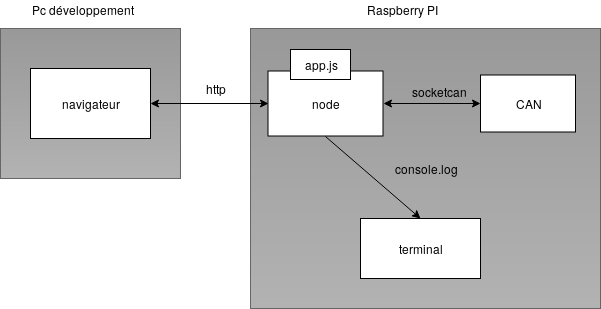
\includegraphics[scale=.5]{./figures-pdf/architecture_logicielle}}
{\caption{architecture logicielle}}
\end{center}
\end{figure}

%terminal distance
\section{Mise en place d’un terminal distant sur la Raspberry Pi}
Pour se connecter à la Raspberry Pi, vous aurez besoin de créer un accès via ssh. Pour cela, depuis un PC d’une salle informatique utilisez la commande :
\begin{verbatim}
ssh pi@10.105.1.x
\end{verbatim} 
avec x.x.x.x: IP addresse de RasPi, qui peut être trouvé par la commande suivant:
\begin{verbatim}
hostname -I
\end{verbatim}
Le mot de passe est : insa.

%exécution et installation
\section{Exécution et installation du serveur nodejs}
Normalement, vous n’aurez pas à configurer et à lancer manuellement le serveur nodejs. Sur chaque Raspberry Pi doit être installé un répertoire UI-CAR contenant l’ensemble de l’application du serveur. Si besoin, pour lancer nodejs manuellement, il faut commencer par se connecter à la Raspberry Pi, puis aller dans le répertoire UI-CAR et lancer la commande 
\begin{verbatim}
node app.js 
(ou simplement ./app.js).
\end{verbatim}
Si le répertoire n’existe pas, il faut récupérer le code sur github en lançant la commande
\begin{verbatim}
git clone https://github.com/daihitsuji/UI-CAR.git
\end{verbatim}
puis installer les dépendances en lançant depuis le répertoire
UI-CAR la commande :
\begin{verbatim}
npm install –save
\end{verbatim}

\section{Connexion au serveur nodejs}
Lancer un navigateur sur un PC et indiquer l’adresse de la raspberry sur le port 3000 dans
la barre d’adresse, par exemple 10.105.1.2 :3000. Vous pouvez ensuite, depuis le moniteur,
lancer différents ordres pour contrôler l’application en cliquant sur les différents boutons ou recevoir les informations de la voiture.


\end{document}